\documentclass[../main.tex]{subfiles}

\begin{document}

\begin{figure}[h!]
	\centering
	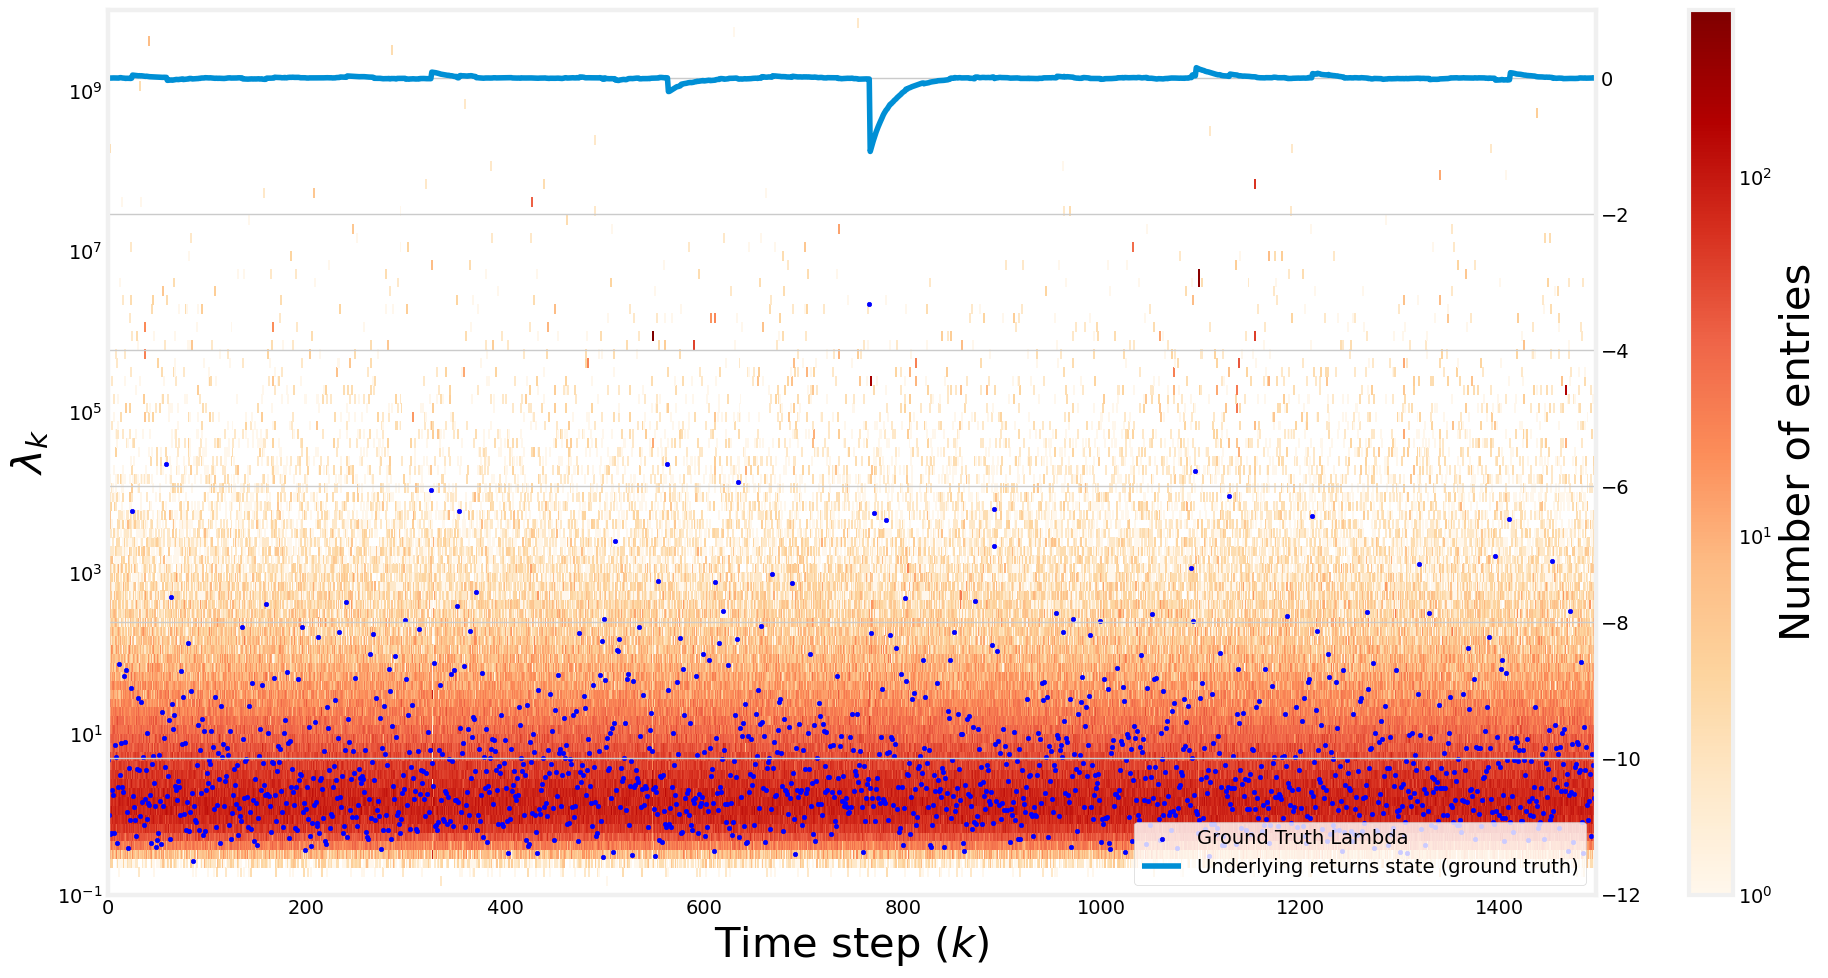
\includegraphics[width=15.0cm]{../plots/4__1__1__lambdas_generic.png}
	\caption{Distribution of samples $\lambda_k^{(i)}$ from the Generic RBPF}
	\label{fig:4__1__1__lambdas_generic}
\end{figure}

\begin{figure}[h!]
	\centering
	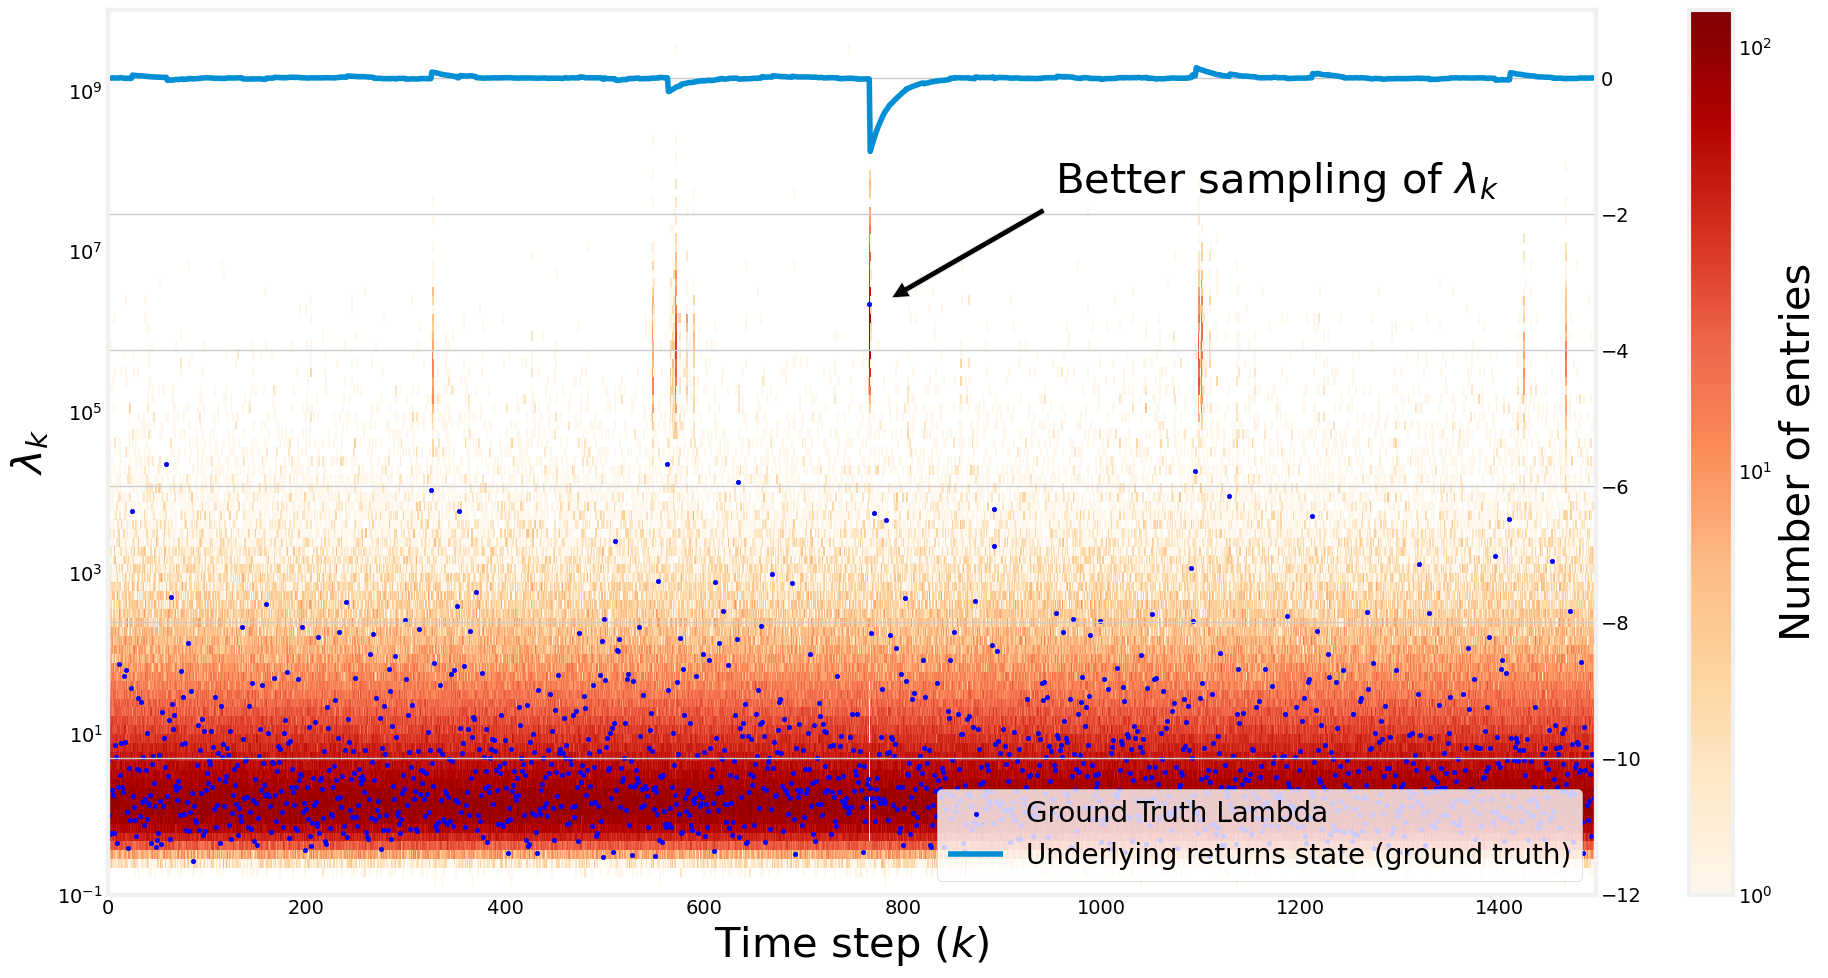
\includegraphics[width=15.0cm]{../plots/4__1__1__lambdas_adaptive_sampling.png}
	\caption{Distribution of samples $\lambda_k^{(i)}$ from the Adaptive Sampling RBPF}
	\label{fig:4__1__1__lambdas_adaptive_sampling}
\end{figure}

Figure \ref{fig:4__1__1__lambdas_generic} shows the distribution of samples $\lambda_k^{(i)}$ from the Adaptive Sampling RBPF as well as the ground truth $\lambda_k$ used to generate the simulation data. 
Figure \ref{fig:4__1__1__lambdas_adaptive_sampling} shows a similar figure for the generic RBPF $\textit{after}$ the resampling step. 

Comparing Figures \ref{fig:4__1__1__lambdas_generic} and \ref{fig:4__1__1__lambdas_adaptive_sampling}, we can see qualitatively that the distribution of samples from the Adaptive Sampling RBPF is distributed more closely around the ground truth $\lambda_k$, resulting in a many more effective samples being generated using the Adaptive Sampling RBPF compared to the generic RBPF.

Note the extremely challenging nature of forming a good importance sampling estimate of the posterior $p(\lambda_k | y_k, \mu_{k-1}, \Sigma_{k-1})$ using only samples from the prior as $\lambda_k$ ranges over 7 orders of magnitude ($10^{-1}$ to $10^7$) in this example. This makes it very difficult to form a good discrete importance sampling estimate, which would require a huge amount of particles to cover the entire possible range of $\lambda_k$ (which theoretically has infinite support). With the adaptive sampling improvement, we are able to use the information from the current observation to sample directly from the approximate posterior, which increases the sampling efficiency of the particle filter greatly. 

We next investigate how few particles we can use with the new adaptive sampling particle filter before performance degrades unacceptably. Figure \ref{fig:4__1__1__very_small_N} shows how the RMSE of the inferred underlying returns process changes for very low values of $N$. Interestingly, we note that the adaptive sampling RBPF is still capable of good inference performance even with extremely low $N = 4$, unlike the generic RBPF, which suffers from degradation of inference performance when using a low number of particles. 

\begin{figure}[h!]
	\centering
	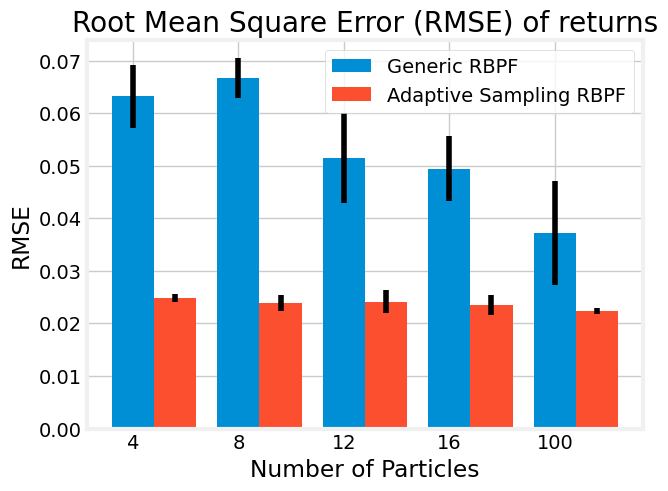
\includegraphics[width=12.0cm]{../plots/4__1__1__very_small_N.png}
	\caption{Performance of the RBPF-based particle filters for very low $N$}
	\label{fig:4__1__1__very_small_N}
\end{figure}

Lastly, we investigate the accuracy and sampling efficiency of our approximate improved rejection sampling method (described in \autoref{sec:adaptive_sampling_RBPF}) that was employed in the adaptive sampling RBPF. 

To investigate the accuracy of the approximate improved rejection sampler, we use the two-sample Kolmogorov–Smirnov(KS) test. The KS test is a two-sided statistical test for the null hypothesis that 2 independent sets of samples are drawn from the same continuous distribution. The KS test statistic quantifies the distance between the empirical distribution function of 2 sets of samples. The smaller the test statistic, the closer the empirical distribution function of these 2 sets of particles. 

Figure \ref{fig:4__1__3__rejection_sampling_ks_test} shows the two-sample KS test statistic obtained when comparing 10000 samples from each of the simple and improved rejection samplers as $\vt$ varies. We note that the KS test statistic is in general very small, and that even at a significance level of $\alpha=0.2$, we are unable to reject the null hypothesis that the 2 sets of samples are different in distribution, demonstrating that our approximate improved rejection sampler is able to produce samples which are close in distribution to the exact simple rejection sampler. 

Figure \ref{fig:4__1__3__rejection_sampling_rej_ratio} shows the rejection ratio of each of the 2 rejection samplers when used to generate 10000 samples. The rejection ratio, defined in \autoref{eq:4__1__3__rejection_ratio}, provides a measure of the sampling efficiency of a rejection sampler by giving an indication of the expected number of iterations needed to draw a single sample from the rejection sampler. For small $\vt$, the improved rejection sampler is equivalent to the original rejection sampler, resulting in roughly similar rejection ratios. However, at large $\vt$, the improved rejection sampler is much more efficient than the simple rejection sampler, and provides large efficiency gains of over 2 orders of magnitude when $\vt$ is large. 

\begin{equation}
	\text{rejection ratio} = \frac{\text{num samples rejected}}{\text{num samples to be generated through rejection sampling}}
	\label{eq:4__1__3__rejection_ratio}
\end{equation}

\begin{figure}[h!]
	\centering
	\subfloat[Two-sample Kolmogorov–Smirnov(KS) Test between simple and improved rejection samplers \label{fig:4__1__3__rejection_sampling_ks_test}]{
		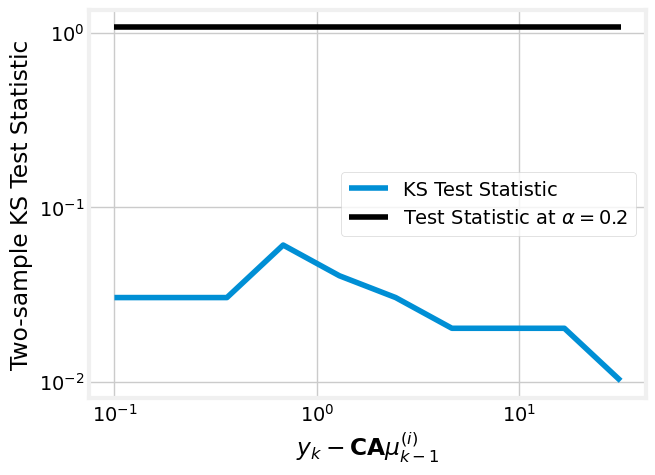
\includegraphics[height=5.5cm]{../plots/4__1__3__rejection_sampling_ks_test.png}}
	\qquad
	\subfloat[Rejection Ratio \label{fig:4__1__3__rejection_sampling_rej_ratio}]{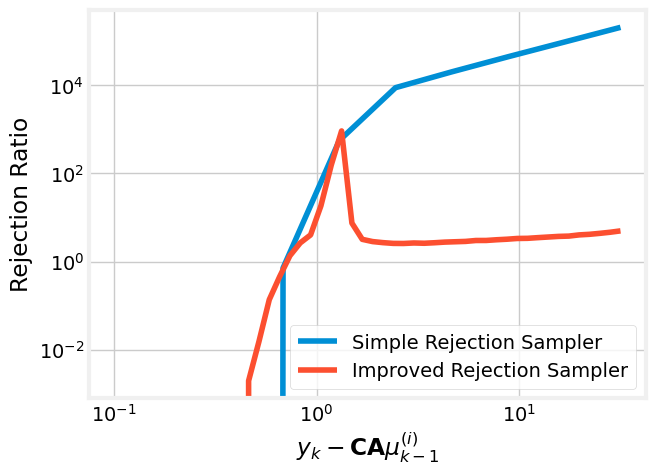
\includegraphics[height=5.5cm]{../plots/4__1__3__rejection_sampling_rej_ratio.png}}
	\caption{Accuracy and sampling efficiency of the improved rejection sampler}
	\label{fig:4__1__3__rejection_sampling}
\end{figure}
	
\end{document}